%
% \iffalse
%<*driver>
\ProvidesFile{xcolor-nyu22.dtx}
%</driver>
%<pkg>\ProvidesPackage{xcolor-nyu22}
%<*pkg>
  [2022/08/10 v0.10.13 Color palettes for the NYU visual identity]
%</pkg>
%<*driver>
\documentclass{ltxdoc}
\usepackage{graphicx}
% \usepackage[letterpaper]{geometry}
\usepackage{xcolor-material}^^A For the \colorsample command
\usepackage{changepage}^^A      For the `adjustwidth' environment

\usepackage{listings}
\lstset{language=bash,basicstyle=\ttfamily}

\usepackage{titling}
\pretitle{\begin{adjustwidth}{0pt}{-1in}\begin{flushleft}\Huge}
\posttitle{\par\end{flushleft}\end{adjustwidth}\vskip 0.5em}
\predate{\begin{flushleft}}
\postdate{\par\end{flushleft}}
\preauthor{\begin{flushleft}}
\postauthor{\par\end{flushleft}}

\usepackage{xcolor-nyu22}

% Set up the NYU primary font families
\usepackage{fontspec}
\setmainfont{Mercury Text G3}
\setsansfont{Gotham Book}

% In the contemporary/subtle tone quadrant, we use sans for the main text
% and serif for the section titles
\renewcommand{\familydefault}{\sfdefault}
\usepackage{titlesec}
\newcommand{\headingfont}{\rmfamily\color{NyuViolet}}
\titleformat*{\section}{\LARGE\headingfont}
\titleformat*{\subsection}{\Large\headingfont}
\titleformat*{\subsubsection}{\large\headingfont}
\renewcommand{\maketitlehooka}{\headingfont}

\usepackage{parskip}



\newlength{\mycontrastboxwidth}
\newcommand{\contrastbox}[5][0.3\linewidth]{%
  \setlength{\mycontrastboxwidth}{#1}%
  \addtolength{\mycontrastboxwidth}{-0.6em}% 
  \colorbox{#3}{%
      \hspace{0.3em}
      \parbox[b][9\baselineskip]{\mycontrastboxwidth}{%
        \normalsize\bfseries\sffamily\color{#2}
        \vspace{0.7em}
        \raggedright{#4}
        \vfill
        \noindent\hfill\Large #5\hfill\hfill\par
        \vfill\vspace{0.7em}}% end of parbox
      \hspace{0.3em}        
  }% end of colorbox
}

\newlength{\paletteunitlength}
\setlength{\paletteunitlength}{0.008\linewidth}
\newcommand{\palettebox}[4]}\vfill}}%
}
\newcommand{\fpalettebox}[5]}\vfill}}%
}

\EnableCrossrefs
\RecordChanges
\CodelineIndex
\usepackage{hyperref}
\begin{document}
  \DocInput{xcolor-nyu22.dtx}
\end{document}
%</driver>
% \fi

% \GetFileInfo{xcolor-nyu22.dtx} 
% \title{The NYU Color Palette}
% \author{Matthew Leingang\thanks{leingang@nyu.edu}} \date{\fileversion, Released \filedate}
% \maketitle

% \begin{abstract}
%  We provide color names for the NYU visual identity.
% \end{abstract}

% \changes{v0.9.0}{2022/08/05}{Added documentation on palette ratios}
% \changes{v0.9.0}{2022/08/02}{Changed package name to \texttt{xcolor-nyu22}} 
% \changes{v0.5.0}{2019/12/13}{Changed package name to \texttt{xcolor-nyu}}
% \changes{v0.4.0}{2019/12/13}{Added documentation}
% \changes{v0.3.2}{2019/12/12}{Split color declaration into a separate package}
% \changes{v0.2.0}{2019/12/11}{Fixed fonts to the official family}
% \changes{v0.1.0}{2019/12/10}{First working release}

% \section{Our Color Palette}
%
% This color palette is from the web page ``NYU Colors'' \cite{NyuColors} from the 
% NYU Brand Kit. A lot of this text is, too.
%
% \textbf{NYU Violet:} NYU Violet is our principal brand color. It should be
% used in every communication and design. Violet is a distinctive color that has
% long been associated with the nonconformist who pushes boundaries to leave
% their mark on the world.
%
% \textbf{Ultra Violet:} An electrified version of NYU Violet, this color adds
% excitement to our communications. Ultra Violet should be used thoughtfully and
% sparingly to add impact or interest, emphasize important information, increase
% contrast, or create rhythm within your design.
%
% \textbf{Black:} A bold color, black strikes the perfect balance between
% sophistication and edginess when used alongside NYU Violet.
%
%
% \section{Color Values} \subsection{Primary Colors}
%
% See Figure~\ref{fig-primary}.
%
% \begin{figure} \centering \colorsample[HTML][13em][White]{NyuViolet}
%   \colorsample[HTML][][White]{UltraViolet} \colorsample[HTML][][White]{Black}
%   \caption{NYU's primary colors} \label{fig-primary} \end{figure}
%
% \subsection{Secondary Colors}
%
% See Figure~\ref{fig-secondary}
%
% \begin{figure} \centering
%     \colorsample[HTML][0.25\textwidth][White]{DeepViolet}
%     \colorsample[HTML][0.25\textwidth][White]{MediumViolet1}
%     \colorsample[HTML][0.25\textwidth][White]{MediumViolet2}
%
%     \colorsample[HTML][0.25\textwidth][White]{LightViolet1}
%     \colorsample[HTML][0.25\textwidth][Black]{LightViolet2}
%     \colorsample[HTML][0.25\textwidth][Black]{White}
%     \caption{NYU's secondary colors. White is actually a neutral 
%     color, but it's included in this table for balance.}
%     \label{fig-secondary}
% \end{figure}
%
% \subsection{Neutral Colors}
%
% See Figure~\ref{fig-neutral}.
%
% \begin{figure} \centering \colorsample[HTML][0.25\textwidth][White]{DarkGray}
%     \colorsample[HTML][0.25\textwidth][White]{MediumGray1}
%     \colorsample[HTML][0.25\textwidth][White]{MediumGray2}
%
%     \colorsample[HTML][0.25\textwidth][Black]{MediumGray3}
%     \colorsample[HTML][0.25\textwidth][Black]{LightGray}
%     \colorsample[HTML][0.25\textwidth][Black]{White}
%
%     \caption{NYU's neutral colors}
%     \label{fig-neutral}
% \end{figure}
%
% \subsection{Accent Colors}
%
% Accent colors can be used for emphasis and contrast within your design. They
% can highlight important elements of your communication such as infographics,
% pull quotes, or even a single word in a title.
%
% This selection of colors gives you the option to add variety to your content
% while working alongside NYU's primary palette. Accent colors are not required,
% but if you want to use one, choose only one and use it sparingly.  See
% Figure~\ref{fig-accents}.
%
% Note that if these color names are already used, this package will overwrite
% them. That is expected behavior, though. The colors are chosen for their
% harmony with the primary colors, so another shade of yellow or blue should not
% be used anyway.
%
% \begin{figure} \centering \colorsample[HTML][5em][White]{Teal}
%    \colorsample[HTML][5em][White]{Magenta}
%    \colorsample[HTML][5em][White]{Blue} \colorsample[HTML][5em][Black]{Yellow}
%    \caption{Accent colors} \label{fig-accents} \end{figure}
%
% \section{Using Color}
%
% \subsection{Palette Ratios}
%
% The color palettes here are suggestions of how to flex the NYU colors to best
% suit the tone of your communication. Not every color in each palette has to be
% used, but NYU Violet should be present in every version of the palette to
% further emphasize the NYU brand.
%
% Our visual tone ranges from \textbf{contemporary to traditional} and
% \textbf{bold to subtle}.  

% \begin{itemize} 
%    \item \textbf{Traditional} visuals often use serif fonts, more detailed
%  graphics, and quieter photography.  
%    \item \textbf{Contemporary} visuals often use sans serif fonts, geometric graphics,
%    and dynamic photography.  
%    \item \textbf{Subtle} visuals include softer colors, toned down graphics, and
%    less-busy photography.  
%    \item \textbf{Bold} visuals are louder, more vibrant, and compositionally energetic. 
% \end{itemize}

% We created a visual tone spectrum with these tones representing the four
% quadrants. You can use this tone spectrum to help you convey a visual tone
% that complements your verbal tone. For more detailed descriptions, refer to
% the Visual Tone Spectrum web page.
%
% These breakdowns are not exact percentages, but they provide an idea of
% relative use. For example, a traditional and subtle design could incorporate
% more NYU Violet than a contemporary and subtle design, and a contemporary and
% bold design could incorporate more black than a contemporary and subtle
% design.
%
% Note: With the exception of headlines, you should set typography primarily in
% black or dark gray. In digital applications, body text should be set to
% \#333333 or \#404040 to reduce the eye strain caused by very high contrast.
%
% \subsubsection{Contemporary/Bold}
%
% The contemporary/bold palette sits in the visual tone spectrum grid's
% top-right quadrant. This tone captures the excitement and energy of urban life
% and NYU's innovative culture. It's a celebration of creative minds in all
% fields coming together to inspire one another, explore possibilities, and
% change the world. This tone is more informal, embracing some of the rougher
% edges and creativity of the city. It resonates most with prospective and
% current students, and alumni.
%
% A beamer slideshow for a club event might use a contemporary/bold tone.
%
% The palette consists of NYU Violet, black, Ultra Violet, Light Violet 1, light
% gray, and white. See Figure~\ref{fig-ratio-contemporary-bold}. 
%
% We used ImageMagick to make a histogram of the colors in the images from 
% \cite{NyuColors}, and rounded the percentages. The shell command was along the
% lines of:
%
% \begin{lstlisting}
% convert file.png \ 
%     -crop "100%x1+230+176" \ 
%     -fuzz "10%" -define histogram:unique-colors=true \ 
%     -format %c histogram:info:- \ 
%     | tr -d ':' | sed -e 's/^    //' | tr ' ' '\t' \  
%     > histogram.tsv
% \end{lstlisting}
%
% This created a tab-separated file suitable for importing into Google spreadsheets.
% From there we could compute the percentages of each color. 
%
% \begin{figure}
%   \centering
%   \palettebox{NyuViolet}{32}{White}{NYU VIOLET}%
%   \palettebox{Black}{32}{White}{BLACK}%
%   \palettebox{UltraViolet}{24}{White}{ULTRA VIOLET}%
%   \palettebox{LightViolet1}{3}{White}{LIGHT VIOLET 1}%
%   \palettebox{LightGray}{3}{Black}{LIGHT GRAY}%
%   \fpalettebox{MediumGray3}{White}{6}{Black}{WHITE}%
%
%   \caption{Palette ratios for the contemporary/bold tone quadrant}
%   \label{fig-ratio-contemporary-bold} 
% \end{figure}
%
% \begin{figure}
%   \centering
%   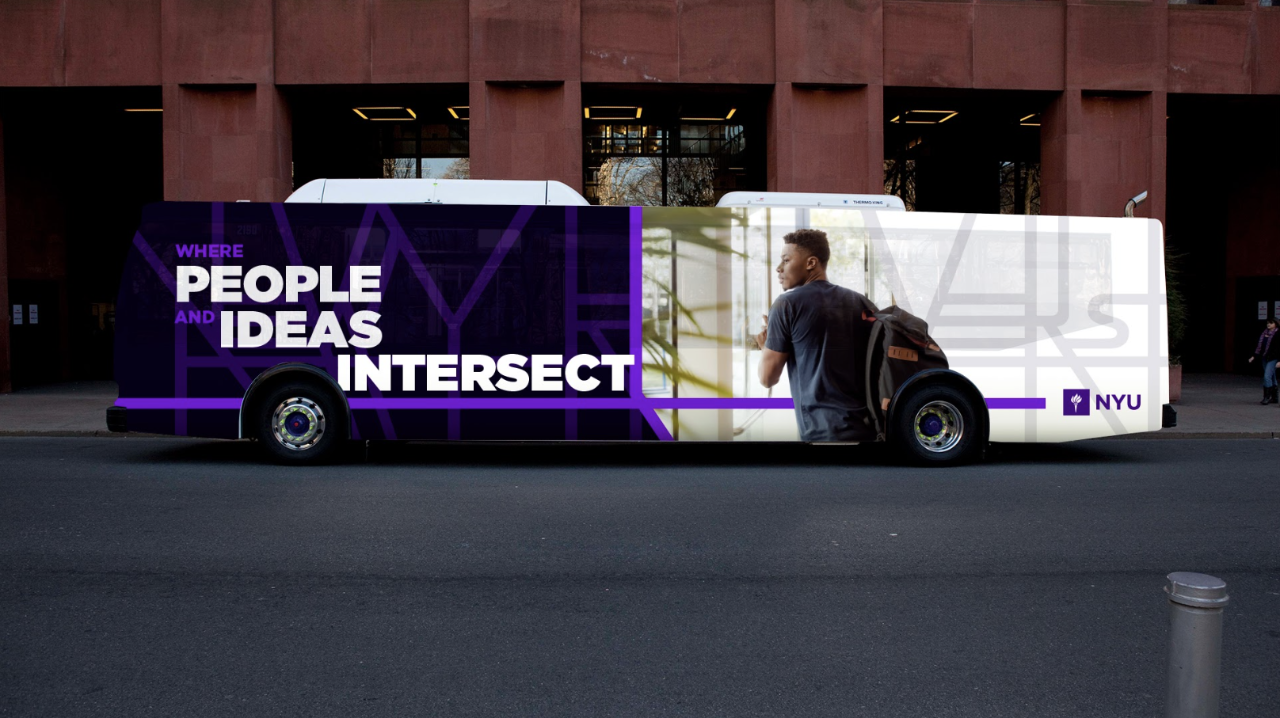
\includegraphics[width=0.8\textwidth]{bus}
%   \caption{Example of the contemporary/bold tone quadrant. Notice the predominance
%     of NYU Violet, black, and ultra violet.}
%   \label{fig-bus}
% \end{figure}
%
%  
% \subsubsection{Contemporary/Subtle}
%
% The contemporary/subtle palette sits in the visual tone spectrum grid's
% top-left quadrant. This tone has the same energy and excitement as
% Contemporary/Bold but is grounded in maturity and confidence. This tone is
% less about getting your attention, and more about rolling up its sleeves and
% getting down to the work required to support the academic mission of the
% University. It resonates more with internal facing audiences like
% administrators, faculty, and staff.
%
% A beamer slideshow for an undergraduate course might use a contemporary/subtle
% tone.
%
% The palette consists of NYU Violet, black, Ultra Violet, medium violet 2,
% light violet 1, light gray, and white. See
% Figure~\ref{fig-ratio-contemporary-subtle}.
%
% \begin{figure}
%   \centering
%   \palettebox{NyuViolet}{15}{White}{NYU VIOLET}%
%   \palettebox{Black}{17}{White}{BLACK}%
%   \palettebox{UltraViolet}{7.5}{White}{ULTRA VIOLET}%
%   \palettebox{MediumViolet2}{7.5}{White}{MEDIUM VIOLET 2}%
%   \palettebox{LightViolet1}{35}{White}{LIGHT VIOLET 1}%
%   \palettebox{LightGray}{3}{Black}{LIGHT GRAY}%
%   \fpalettebox{MediumGray3}{White}{15}{Black}{WHITE}%
%
%   \caption{Palette ratios for the contemporary/subtle tone quadrant}
%   \label{fig-ratio-contemporary-subtle}
% \end{figure}
%
%
% \subsubsection{Traditional/Bold}
%
% The traditional/bold palette sits in the visual tone spectrum grid's
% bottom-right quadrant. This tone is for matter-of-fact or hard-fact messaging
% that needs the weight of NYU's gravitas behind it. It conveys a sense of
% importance, so consider it for quieter, more reserved pieces. It resonates
% with more mature audiences like retired faculty, graduate students, and
% external financial partners.
%
% An undergraduate exam might use this tone.
%
% The palette consists of NYU Violet, deep violet, Ultra Violet, medium violet
% 2, light violet 1, and white.  See Figure~\ref{fig-ratio-traditional-bold}.
%
% \begin{figure}
%   \centering
%   \palettebox{NyuViolet}{40}{White}{NYU VIOLET}%
%   \palettebox{DeepViolet}{18}{White}{DEEP VIOLET}%
%   \palettebox{UltraViolet}{7.5}{White}{ULTRA VIOLET}%
%   \palettebox{MediumViolet2}{18}{White}{MEDIUM VIOLET 2}%
%   \palettebox{LightViolet1}{7.5}{White}{LIGHT VIOLET 1}%
%   \fpalettebox{MediumGray3}{White}{9}{Black}{WHITE}%
%
%   \caption{Palette ratios for the traditional/bold tone quadrant}
%   \label{fig-ratio-traditional-bold} \end{figure}
%
%
% \subsubsection{Traditional/Subtle}
%
% The traditional/subtle palette sits in the visual tone spectrum grid's
% top-left quadrant. This tone is for formal communications that require a
% personal and accessible touch. Grounded in tradition, it is sophisticated and
% restrained, and it emphasizes our position as a prestigious academic
% institution. It resonates with most donors, trustees, and audiences of formal
% events like commencement.
%
% Class notes in article format might use a traditional/subtle tone. The same
% could be said about the documentation files for this bundle.
%
% The palette consists of NYU Violet, black, Ultra Violet, medium violet 2,
% light violet 1, light gray, and white. See
% Figure~\ref{fig-ratio-traditional-subtle}.
%
% \begin{figure}
%   \centering
%   \palettebox{NyuViolet}{40}{White}{NYU VIOLET}%
%   \palettebox{DeepViolet}{18}{White}{DEEP VIOLET}%
%   \palettebox{LightViolet1}{7}{White}{LIGHT VIOLET 1}%
%   \palettebox{MediumGray2}{7}{Black}{MEDIUM GRAY 2}%
%   \palettebox{LightGray}{7}{Black}{LIGHT GRAY}%
%   \fpalettebox{MediumGray3}{White}{21}{Black}{WHITE}%
%
%   \caption{Palette ratios for the traditional/subtle tone quadrant}
%   \label{fig-ratio-traditional-subtle}
% \end{figure}
%
%
% \subsection{Palette Ratio Examples}
%
% The bus wrap in Figure~\ref{fig-bus} shows a graphic in the contemporary/bold
% quadrant. It's not really possible to verify the percentages, but you can See
% the predominance of the NYU Violet, black, and ultra violet.
%
% \section{Accessibility}
%
% \subsection{Color Contrast}
%
% Color contrast is the difference between two colors. If the foreground colors
% of visual elements are too similar to the background colors, it can be
% difficult for people to read or understand. Be sure to check the color
% contrast between your text and background colors to ensure your message is
% legible.
%
% Text should have a contrast ratio of at least 3-to-1. According to the World
% Wide Web Consortium, if icons are required to understand content, then they
% must also have a contrast ratio of at least 3-to-1. There are many resources
% available, such as the WAVE tool, to check the color contrast in your designs.
% See Figures \ref{fig-high-contrast}~and~\ref{fig-low-contrast}.
%
% \begin{figure}
% \begin{adjustwidth}{-1in}{-1in}
% \contrastbox{White}{NyuViolet}{11.6:1}{High Contrast}
% \contrastbox{DarkGray}{LightGray}{9.6:1}{High Contrast}
% \contrastbox{White}{UltraViolet}{6.7:1}{High Contrast}
% \end{adjustwidth}
% \caption{High contrast combinations of the NYU color palette}
% \label{fig-high-contrast}
% \end{figure}
%
% \begin{figure}
% \begin{adjustwidth}{-1in}{-1in}
% \contrastbox{UltraViolet}{NyuViolet}{1.7:1}{Low Contrast}
% \contrastbox{NyuViolet}{Black}{1.6:1}{Low Contrast}
% \contrastbox{NyuViolet}{UltraViolet}{1.7:1}{Low Contrast}
% \end{adjustwidth}
% \caption{Low contrast combinations of the NYU color palette. These should be avoided.}
% \label{fig-low-contrast}
% \end{figure}
%
%
% \bibliographystyle{plain}
% \bibliography{xcolor-nyu22}
%
% \StopEventually{\PrintChanges}
%
% \section{Implementation}
%
%    \begin{macrocode}
%<*pkg>
\RequirePackage{xcolor}
%    \end{macrocode}
%
%
% Violets
%
% \changes{v0.9.0}{2022/08/03}{Changed the primary name from \texttt{nyupurple} to \texttt{NyuViolet}}
% \changes{v0.9.0}{2022/08/03}{Added \texttt{UltraViolet} and \texttt{Black}}
% \changes{v0.9.0}{2022/08/03}{Added the medium and light violets}
%    \begin{macrocode}
\definecolor{NyuViolet}{HTML}{57068C}
\definecolor{UltraViolet}{HTML}{8900e1}
\definecolor{Black}{HTML}{000000}% none more black
\definecolor{DeepViolet}{HTML}{330662}
\definecolor{MediumViolet1}{HTML}{702b9d}
\definecolor{MediumViolet2}{HTML}{7b5aa6}
\definecolor{LightViolet1}{HTML}{ab82c5}
\definecolor{LightViolet2}{HTML}{eee6f3}
% deprecated
\colorlet{nyupurple}{NyuViolet}
\colorlet{nyupurple1}{NyuViolet}
\definecolor{nyupurple2}{HTML}{8900E1}
\definecolor{nyupurple3}{HTML}{330062}
\definecolor{nyupurple4}{HTML}{220337}
%    \end{macrocode}
%
% Blacks and grays
% \changes{v0.9.0}{2022/08/03}{Added the 2022 gray shades and deprecated the prior ones}
%    \begin{macrocode}
\definecolor{DarkGray}{HTML}{404040}
\definecolor{MediumGray1}{HTML}{6d6d6d}
\definecolor{MediumGray2}{HTML}{b8b8b8}
\definecolor{MediumGray3}{HTML}{d6d6d6}
\definecolor{LightGray}{HTML}{f2f2f2}
\definecolor{White}{HTML}{ffffff}
% deprecated color names
\definecolor{nyugblack}{HTML}{000000}
\definecolor{nyugray}{HTML}{6D6D6D}
\colorlet{nyugray1}{nyugray}
\definecolor{nyugray2}{HTML}{B8B8B8}
\definecolor{nyugray3}{HTML}{D6D6D6}
\definecolor{nyugray4}{HTML}{F2F2F2}
%    \end{macrocode}
%
% Accent colors
%
% \changes{v0.9.0}{2022/08/03}{Added the 2022 accent colors and deprecated the prior alert ones}
%
%    \begin{macrocode}
\definecolor{Teal}{HTML}{009b8a}
\definecolor{Magenta}{HTML}{fb0f78}
\definecolor{Blue}{HTML}{59B2D1}
\definecolor{Yellow}{HTML}{f4ec51}
% deprecated
\definecolor{nyured}{HTML}{CB0200}% warning
\definecolor{nyuorange}{HTML}{E86C00}% info
\definecolor{nyugreen}{HTML}{489141}% success
%    \end{macrocode}
%
% Tertiary accent colors
%
%    \begin{macrocode}
% deprecated
\definecolor{nyudarkblue}{HTML}{28619E}
\colorlet{nyuaccent1}{nyudarkblue}
\definecolor{nyulightblue}{HTML}{3DBBDB} 
\colorlet{nyuaccent1}{nyulightblue}
\definecolor{nyuteal}{HTML}{007C70}
\colorlet{nyuaccent3}{nyuteal}
\definecolor{nyupink}{HTML}{D71E5E}
\colorlet{nyuaccent4}{nyupink}
\colorlet{nyuaccent5}{nyuorange}
\definecolor{nyuyellow}{HTML}{FFC107}
\colorlet{nyuaccent6}{nyuyellow}
%    \end{macrocode}
%
%    \begin{macrocode}
%</pkg>
%    \end{macrocode}
%
% \Finale
%
